\begin{figure}
	\centering
	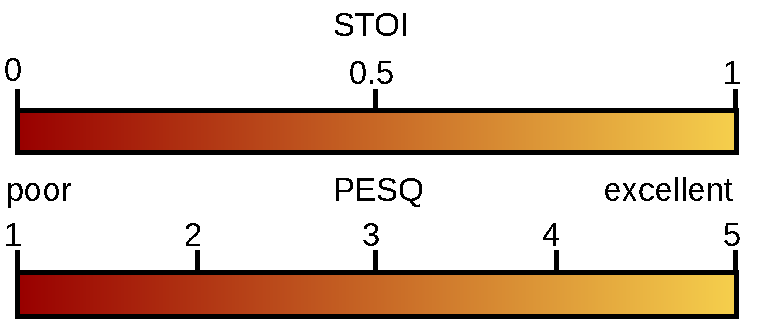
\includegraphics[width=0.5\textwidth]{metrics}
	\caption{\ac{PESQ} and \ac{STOI} metric scales}
	\label{fig:metrics}
\end{figure}

\begin{table}
	\centering
	\caption{mean change STOI and PESQ scores for a subset of the validation set}
	\label{tab:results}
	\resizebox{0.5\textwidth}{!} {
	\begin{tabular}{lrr}
	\toprule
			  Method &  avg. $\Delta$STOI &  \ avg. $\Delta$PESQ \\
	\midrule
	Frequency-domain &         0.070 &        -0.383 \\
		 Time-domain &         0.023 &        -0.159 \\
	\bottomrule
	\end{tabular}
	}
\end{table}

To evaluate the results, two common speech metrics are used: \ac{STOI} and \ac{PESQ}. \ac{STOI} measures speech intelligibility, whereas \ac{PESQ} measures speech quality. Figure \ref{fig:metrics} shows the scaling for each score.Table \ref{tab:results} shows the mean change in the speech metric scores for 10 random reconstructed examples from the validation set. Both the time-domain and frequency-domain networks improve the \ac{STOI} while making the \ac{PESQ} worse. These networks may be useful for tasks such as \ac{ASR} where intelligibility is valued over quality. Notably, the frequency-domain network achieved both a larger boost in \ac{STOI} and a larger detriment to the \ac{PESQ} than the time-domain network. Figure \ref{fig:specs} shows spectrograms for the input, target, and both models for an example speech sequence.

\begin{figure}
	\centering
	\includegraphics[width=0.5\textwidth]{../../project/figs/specs2}
	\caption{Spectrograms of Reconstructed Example}
	\label{fig:specs}
\end{figure}
